\documentclass{sprawozdanie-agh}
\usepackage[utf8]{inputenc}
\usepackage[figurename=Wykres,tablename=Tabela]{caption}
\usepackage[table]{xcolor}
\renewcommand\thefigure{\arabic{figure}.}
\renewcommand\thetable{\arabic{table}.}
\titlespacing*{\subsubsection} {0pt}{1ex plus 1ex minus .2ex}{0.2ex plus .2ex}
\usepackage{titlesec}
\usepackage{footnote}
\makesavenoteenv{tabular}
\makesavenoteenv{table}
\usepackage{graphicx}
\usepackage{array}
\usepackage{makecell}
\usepackage{titlesec}
\usepackage{indentfirst}
\usepackage{booktabs}
\usepackage{forest}
\usepackage{xcolor}
\usepackage{mandi}
\usepackage{listings}
\definecolor{fond}{RGB}{246,246,246}
\definecolor{lightgray}{gray}{0.5}
\newcommand{\dtoprule}{\specialrule{1pt}{0pt}{0.4pt}%
            \specialrule{0.3pt}{0pt}{\belowrulesep}%
            }
\newcommand{\dbottomrule}{\specialrule{0.3pt}{0pt}{0.4pt}%
            \specialrule{1pt}{0pt}{\belowrulesep}%
            }
%\titleformat*{\subsection}{\large\bfseries}
\newcolumntype{x}[1]{>{\centering\arraybackslash}p{#1}}
\usepackage{tikz}
\titlelabel{\thetitle.\quad}
\renewcommand{\thesection}{\Roman{section}}
\renewcommand{\thesubsection}{\thesection.\Alph{subsection}}
\makeatletter
\newcommand\blfootnote[1]{%
  \begingroup
  \renewcommand\thefootnote{}\footnote{#1}%
  \addtocounter{footnote}{-1}%
  \endgroup
}
\titlespacing* % starred version: first paragraph is not indented
    {\subsection} % <command>
    {0em} % <left>
    {1ex plus 0.5ex minus .1ex} % <before-sep>
    {0.5ex plus .1ex} % <after-sep>
\begin{document}
\lstset{
	language=make,%
	inputencoding=utf8,%x-iso-8859-15,%
	extendedchars=true,%
	basicstyle=\tiny\ttfamily, % Standardschrift
	numberstyle=\tiny\color{gray},
	keywordstyle=\color{orange},
	commentstyle=\color{teal},
	stringstyle=\color{red},
    identifierstyle=\color{blue},
	numbers=left,               % Ort der Zeilennummern
	numberstyle=\tiny\color{gray}, % Stil der Zeilennummern
	%	stepnumber=2,               % Abstand zwischen den Zeilennummern
	numbersep=5pt,              % Abstand der Nummern zum Text
	tabsize=2,                  % Groesse von Tabs
	breaklines=true,            % Zeilen werden Umgebrochen
	frame=tb,         
	showspaces=false,           % Leerzeichen anzeigen ?
	showtabs=false,             % Tabs anzeigen ?
	xleftmargin=17pt,
	framexleftmargin=17pt,
	framexrightmargin=0pt,
	framexbottommargin=2pt,
	backgroundcolor=\color{fond},
	showstringspaces=false,     % Leerzeichen in Strings anzeigen ?   
	literate={@}{{\textcolor{green}{@}}}{1}   
    		 {ą}{{\k{a}}}1
             {Ą}{{\k{A}}}1
             {ę}{{\k{e}}}1
             {Ę}{{\k{E}}}1
             {ó}{{\'o}}1
             {Ó}{{\'O}}1
             {ś}{{\'s}}1
             {Ś}{{\'S}}1
             {ł}{{\l{}}}1
             {Ł}{{\L{}}}1
             {ż}{{\.z}}1
             {Ż}{{\.Z}}1
             {ź}{{\'z}}1
             {Ź}{{\'Z}}1
             {ć}{{\'c}}1
             {Ć}{{\'C}}1
             {ń}{{\'n}}1
             {Ń}{{\'N}}1
}

\przedmiot{Metody i Narzędzia Programowe w Akustyce}
\tytul{Projekt MES}
\podtytul{Obliczenia charakterystyk straty wtrącenia akustycznego tłumika refleksyjnego oraz optymalizacja geometrii kanału}
\kierunek{Inżynieria Akustyczna}
\autor{\textbf{Grupa 3, III rok}\\Maja Szydłowska,\\Justyna Szymańska,\\Dominika Woźniak,\\Alexander Stefani}
\data{Kraków, 15 czerwca 2020}

\stronatytulowa{}
\section{Wstęp}
\par Przedmiotem projektu jest analiza tłumika refleksyjnego o wymiarach stałych i schemacie przekroju opisanym na \hyperref[rysunek]{rysunku 1.} Zakres wymiarów sparametryzowanych jako zmienne wejściowe jest przedstawiony w \hyperref[tabela]{tabeli 1.} wraz analizowanym pasmem częstotliwości.
\par Zadaniem grupy było dokonanie obliczeń charakterystyki częstotliwościowej straty wtrącenia opisanego tłumika kołowego w pakiecie obliczeniowym do metody elementów skończonych -- Elmer FEM, który posiada moduł dla akustycznego równania Helmholtza.
\par Następnie, zgodnie z wybranym przez grupę planem eksperymentu opisanym poniżej, zostały wyznaczone charakterystyki straty wtrącenia dla zmiennych wejściowych, które metodą optymalizacji dadzą średnice kanałów: $x_1$, $x_2$ tłumika o największej całkowitej stracie wtrącenia w zadanym paśmie częstotliwości, metodą omiatania częstotliwościami (scanning).
\par Porównawczo, zastosowano metodę omiatania parametrów wejściowych z małym krokiem dyskretyzacji (sweep) w celu uzyskania precyzyjnych wyników. Jest ona potrzebna do weryfikacji poprawności planu eksperymentu, który w naszej grupie uległ modyfikacji opisanej niżej.
\begin{figure}[ht]
\vspace{-0.6cm}
    \centering
\scalebox{1.7}{
\tikzset{every picture/.style={line width=0.75pt}} %set default line width to 0.75pt        
\tikzstyle{loosely dashdotted}=      [dash pattern=on 3pt off 4pt on \the\pgflinewidth off 4pt]
\begin{tikzpicture}[x=0.75pt,y=0.75pt,yscale=-1,xscale=1]
%uncomment if require: \path (0,132); %set diagram left start at 0, and has height of 132

%Straight Lines [id:da2966962714614121] 
\draw [line width=1.5]    (50,86.16) -- (50,128) ;
%Straight Lines [id:da3063968048761292] 
\draw [line width=1.5]    (79.5,86.16) -- (20.5,86.16) ;
%Straight Lines [id:da8939199304798044] 
\draw [line width=1.5]    (79.5,64.16) -- (20.5,64.16) ;
%Straight Lines [id:da8682181187399829] 
\draw [line width=1.5]    (50,22.31) -- (50,64.16) ;
%Straight Lines [id:da47356084160708756] 
\draw [line width=1.5]    (20.5,64.16) -- (20.5,55.31) ;
%Straight Lines [id:da6368950626113001] 
\draw [line width=1.5]    (20.5,95) -- (20.5,86.16) ;
%Straight Lines [id:da5398079529412676] 
\draw [color={rgb, 255:red, 155; green, 155; blue, 155 }  ,draw opacity=1 ][line width=1.5]    (20.5,64.16) -- (20.5,86.16) ;

%Straight Lines [id:da20265780718260173] 
\draw [line width=1.5]    (50,22.31) -- (196.29,22.31) ;
%Straight Lines [id:da01791161396808527] 
\draw [line width=1.5]    (50,128) -- (196.29,128) ;
%Straight Lines [id:da8212902519436587] 
\draw [line width=1.5]    (196,64.16) -- (196,22.31) ;
%Straight Lines [id:da19255605999705994] 
\draw [line width=1.5]    (196,128) -- (196,86.16) ;
%Straight Lines [id:da5385843807099637] 
\draw [line width=1.5]    (255,86.16) -- (255,95) ;
%Straight Lines [id:da501625921928528] 
\draw [line width=1.5]    (255,55.31) -- (255,64.16) ;
%Straight Lines [id:da5236755672880284] 
\draw [color={rgb, 255:red, 155; green, 155; blue, 155 }  ,draw opacity=1 ][line width=1.5]    (255,86.16) -- (255,64.16) ;
%Straight Lines [id:da9330741448584701] 
\draw  [loosely dashdotted]  (104,75.16) -- (3.29,75.16) ;
%Straight Lines [id:da8091423567938218] 
\draw  [loosely dashdotted]  (193.5,75.16) -- (123.14,75.16) ;
%Straight Lines [id:da939584502120711] 
\draw  [loosely dashdotted]  (104,75.16) -- (10.29,75.16) ;
%Straight Lines [id:da9014678298103178] 
\draw   [<->] (123.14,128) -- (123.14,22.31) ;

%Straight Lines [id:da4291514999716699] 
\draw  [<->]  (210,86) -- (210,64);
%Straight Lines [id:da9625264551828747] 
\draw [<->]    (50,11.31) -- (196,11.31) ;
%Straight Lines [id:da46897335301217025] 
\draw    (50,8) -- (50,22.31) ;
%Straight Lines [id:da6799153240429547] 
\draw    (196,8) -- (196,22.31) ;

%Straight Lines [id:da7597687766897696] 
\draw [<->]    (50,53.31) -- (79.5,53.31) ;
%Straight Lines [id:da733666892111086] 
\draw    (79,50) -- (79,64.31) ;
%Straight Lines [id:da25885199121376035] 
\draw [<->]    (167,53.31) -- (196,53.31) ;

%Straight Lines [id:da8954781024642482] 
\draw    (167.5,50) -- (167.5,64.31) ;
%Straight Lines [id:da07715896931159993] 
\draw  [loosely dashdotted]  (275,75.16) -- (215,75.16) ;
%Straight Lines [id:da20774439044915138] 
\draw [line width=1.5]    (166.5,86.16) -- (255,86.16) ;
%Straight Lines [id:da04509401303207716] 
\draw [line width=1.5]    (167,64.16) -- (255,64.16) ;

% Text Node
\draw (110.9,82.81) node [anchor=north west][inner sep=0.75pt]  [font=\tiny,rotate=-270]  {$0,6$};
% Text Node
\draw (197.9,82.81) node [anchor=north west][inner sep=0.75pt]  [font=\tiny,rotate=-270]  {$0,1$};
% Text Node
\draw (118.5,0.21) node [anchor=north west][inner sep=0.75pt]  [font=\tiny]  {$x_{2}$};
% Text Node
\draw (59.5,43.21) node [anchor=north west][inner sep=0.75pt]  [font=\tiny]  {$x_{1}$};
% Text Node
\draw (176.5,43.21) node [anchor=north west][inner sep=0.75pt]  [font=\tiny]  {$x_{1}$};
\end{tikzpicture}}
    \renewcommand{\figurename}{Rys.}
    \caption{Schemat przekroju tłumika refleksyjnego dla grupy 3.}
    \label{rysunek}
\end{figure}
\vspace{-0.2cm}
\begin{table}[ht]
\centering
    \caption{Zakres parametrów wejściowych oraz kroki dyskretyzacji dla metody omiatania}
    \label{tabela}{
\begin{tabular}{c|r|r|r}
\rowcolor{gray!30} Parametr & \multicolumn{1}{|c|}{Minimum} & \multicolumn{1}{|c|}{Maksimum} & \multicolumn{1}{|c}{\begin{tabular}[c]{@{}c@{}}Krok\\ dyskretyzacji\end{tabular}} \\  \dbottomrule
$x_1$ {[}m{]} & 0,05 & 0,4 & 0,05 (sweep) \\ \midrule
$x_2$ {[}m{]} & 0,2  & 1,0 & 0,1 (sweep) \\ \midrule
$f$ {[}Hz{]}  & 100  & 500 & 1 (CCI/\textbf{sweep\footnote{Dało to aż 17 644 par symulacji MES, ale dzięki temu, nie ma problemu z aliasingiem częstotliwości.}}) \\ \dbottomrule
\end{tabular}}
\end{table}
\vspace{-0.4cm}
\subsection{Problemy}
\subsubsection{Wybór planu eksperymentu}
    Jak widać na \hyperref[rysunek]{rys. 1.}, fizyczny warunek na istnienie tłumika zachodzi, gdy parametry spełniają nierówność: $x_2> 2 x_1$, inaczej współrzędne siatki MES nie miałyby rosnących wartości, a kanał tłumika zostałby zamknięty. To znacznie ogranicza zakres parametrów wejściowych, które rozplanowane na planie kompozycyjnym dadzą mniej punktów do interpolacji funkcji modelu zastępczego (powierzchnia odpowiedzi). To dało w rzeczywistości 6 z 9 możliwych punktów na planie kompozycyjnym zarówno CCI jak i CCC.\newpage \vspace{-0.6cm}
\subsubsection{Wyznaczanie parametru modelu zastępczego}
    Dodatkowym problemem jest brak zdefiniowanej ogólnej funkcji celu dla powierzchni odpowiedzi, ponieważ strata wtrącenia $IL(f)$ jest charakterystyką częstotliwościową \hyperref[ref1]{[1]}.\\Nie można zatem wykonać jednego planu eksperymentu dla całego pasma częstotliwości, należy przyjąć jakąś funkcję zastępczą dającą opisać się na całym przedziale. \\ Wykluczono natomiast możliwość filtrowania charakterystyki w pasmach tercjowych/oktawowych i wyznaczania $n$-planów eksperymentu (gdzie $n$ to liczba pasm), ponieważ celem zadania nie było przeprowadzenie optymalizacji tłumika dla wybranych arbitralnie częstotliwości, a dla całego pasma.
    \subsubsection{Długość wlotu i wylotu oraz wektor współrzędnych $X$ domen siatki}
    Jak widać z \hyperref[rysunek]{rysunku 1.}, zadana geometria kanału wlotu jak i wlotu nie jest przedstawiona w skali odnosząc się do $x_1$ i $x_2$. Nie zostało jednak powiedziane jaka powinna być stała długość wlotu i wylotu, więc grupa przyjęła długość wlotu na \textbf{5 m}, a wylotu na \textbf{10~m}, proporcjonalnie do stosunku ich długości na rysunku. Aby wlot i wylot nie miały dużego wpływu na zjawiska falowe w tłumiku, ich długość musi być znacznie większa od największej długości fali rozpatrywanej w paśmie -- (jest to dla 100 Hz: 3,43 m), więc warunek został spełniony. Zgodnie z \hyperref[ref1]{[1]}, przyjęto fizyczną grubość ścianek = 1 cm.
    \par Aby ułatwić obliczenia wartości ciśnienia dla wylotu, przyjęto środek układu współrzędnych siatki (0,0) jako koniec wylotu położony w środku symetrii kanału tłumika.
\subsection{Rozwiązania:}
\subsubsection{Ad A.1.}
Grupa zaproponowała jako rozwiązanie zastosowanie uboższego \textbf{planu eksperymentu CCI (6-punktowego)}, rozszerzonego o walidację z dokładnymi wartościami interpolowanej powierzchni odpowiedzi metodą omiatania po wszystkich parametrach wejściowych z~małym krokiem. Odbywa się to kosztem czasu obliczeń symulacji MES, natomiast daje pełną informację o punktach pośrednich między punktami planu eksperymentu. Początkowo wybrano plan CCC, który zgodnie z \hyperref[ref2]{[2]}: ,,pozwala na uzyskanie wysokiej jakości dopasowania powierzchni odpowiedzi w całym badanym obszarze'', niestety zakres parametrów wejściowych przekracza przedział nieujemnych (fizycznych) wartości, więc porzucono ten plan.
\subsubsection{Ad A.2.} Aby uzyskać funkcję całkowitej straty wtrącenia w artykułach o tłumieniu przegród dźwiękochłonnych znaleziono inną definicję na stratę wtrącenia $IL$ \textit{(insertion loss)} \hyperref[ref3]{[3]},~\hyperref[ref4]{[4]}. Jest to \textbf{poziom stosunku mocy całkowitych:} źródła dźwięku do wypromieniowywanej za odgrodą tłumiącą. Dzięki temu, definicja ta jest prostsza w naszym problemie, ponieważ należy wyznaczyć dla każdej pary tłumik-falowód estymaty całkowitych mocy akustycznych.
\begin{align*}
    \textrm{Zgodnie z definicją mocy akustycznej:}\quad&P=\tfrac{I}{S}=\tfrac{\left\langle p^2\right\rangle}{Z S}\\
    \textrm{oraz definicją na moc ,,fizyczną'':}\quad&P=\tfrac{E_{tot}}{\Delta t}=E_{tot}\Delta f=\textstyle\sum\nolimits_i E(f[i]) \Delta f
\end{align*}
-- można wywnioskować, że bardzo dobrą estymatą mocy całkowitej będzie całka (dyskretna suma) w zadanym paśmie częstotliwości, pod warunkiem, że źródło dźwięku będzie wypromieniowywać stałą gęstość mocy widmowej, ale tylko w tym paśmie częstotliwości.\\ Jako, że impedancja właściwa $Z$ oraz średnica przekroju $S$ nie zmienią się, całkowita strata wtrącenia będzie poziomem stosunku mocy całkowitych wypromieniowywanych przez falowód płaski i tłumik akustyczny (całek z uśrednionych kwadratów amplitud ciśnienia $\left\langle p^2\right\rangle$ przy wylocie, czyli energii):
\vspace{-0.7cm}
\begin{equation}
     \boxed{IL_{tot} = 10\log_{10}{\frac{\sum_i \left\langle p_{\textrm{bez}}^2[i] \right\rangle\Delta f}{\sum_i \left\langle p_{\textrm{tłum}}^2[i]\right\rangle \Delta f}}  }
     \label{eq}
\end{equation}
\section{Algorytm obliczeniowy}
\subsection{Opis działania}
Jako, że grupa dostała tłumik geometrycznie podobny do tłumika opisanego na laboratorium, w niniejszej pracy nie będzie ponownie przedstawiana struktura domen obliczeniowych siatki, a grupa odsyła do rysunku w punkcie \textbf{4.1. konspektu do lab. 2.} \hyperref[ref1]{[1]}.
\par W celu wykonywania algorytmu i wywoływania podprogramów, wybrano napisanie głównego skryptu \texttt{\hyperref[list1]{runmuffler.sh}} dla powłoki systemowej Linuxa -- \texttt{Bash} oraz dokonywanie obliczeń macierzowych i interpolacji w~skryptach pakietu \texttt{Octave}: \texttt{\hyperref[list5]{replace.m}} -- tworząca wektor siatki na osi $X$, \texttt{\hyperref[list7]{cci.m}} -- wyznaczająca punkty planu CCI i  \texttt{\hyperref[list6]{optimize.m}} -- opisana dalej.\\ Kluczem do prostoty obliczeń jest automatyzacja podmieniania parametrów wejściowych w~plikach: \textbf{siatki tłumika --} \texttt{\hyperref[list2]{tlumik.grd}}, \textbf{siatki płaskiego falowodu --} \texttt{\hyperref[list3]{plaski.grd}} oraz \textbf{solvera} \texttt{ElmerSolver} -- \texttt{\hyperref[list4]{case.sif}}, dokonywana wyrażeniem regularnym \texttt{\color{orange}sed} na znaku \texttt{\color{green}@}.\\
Lokalizacja szablonów tekstowych dla plików \texttt{case.sif},\texttt{tlumik.grd}, \texttt{plaski.grd} znajduje się podfolderze \texttt{./data}.
\par Punkty należące do zbioru punktów ,,fizycznych'' zwraca skrypt \hyperref[list7]{\texttt{cci.m}} do pliku tekstowego \texttt{cci-t1t2.txt}, następnie główny skrypt wykonawczy \texttt{\hyperref[list1]{runmuffler.sh}} najpierw konwertuje pliki wyników symulacji MES -- \texttt{output.dat} do plików:\\\texttt{cci-tlumik.txt}, \texttt{cci-plaski.txt} z wartościami oddzielonymi przecinkami,  ulokowane w~folderach: \texttt{./output/tlumik}, \texttt{./output/plaski}, dopiero wtedy funkcja \hyperref[list6]{\texttt{optimize.m}} pobiera wektory współrzędnych planu CCI z \texttt{cci-t1t2.txt}, sortuje wyniki symulacji MES z poprzednio sformatowanych plików tekstowych i przeprowadza optymalizację.
\par Dodatkowo stworzono podfunkcję \texttt{\hyperref[list8]{sortcalc.m}} wykonującą bezpośrednio sortowanie wyników z zadanych plików do macierzy i wyznaczanie $IL_{tot}$, by zwrócić je do funkcji \hyperref[list6]{\texttt{optimize.m}}.
\subsection{Schemat algorytmu}
\par Schemat procedury obliczeniowej znajduje się na \hyperref[rysunek2]{rysunku 2}, a listingi plików pod nim. Jako poprawne wywołanie \texttt{\hyperref[list1]{runmuffler.sh}} z poziomu \texttt{Bash}'a podaje się po nazwie argumenty kroków dyskretyzacji: $\Delta x_1, \Delta x_2, \Delta f$, zgodnie z notacją:\\
\texttt{./runmuffler.sh [krok\_x1] [krok\_x2] [krok\_f] [CCI|SWEEP]}(2 flagi boolean)\\
Dodatkowo wstawiając logiczną flagę po argumentach, np. \texttt{01}, można wybrać, że moduł MES ma nie obliczać danych z punktów CCI, a tylko z omiatania parametrami $x_1,x_2$.
\begin{figure}[ht]
    \centering
\scalebox{1.2}{
\tikzset{every picture/.style={line width=0.75pt}} %set default line width to 0.75pt        
\begin{tikzpicture}[x=0.75pt,y=0.75pt,yscale=-1,xscale=1]
%uncomment if require: \path (0,200); %set diagram left start at 0, and has height of 200
%Rounded Rect [id:dp9743873851957945] 
\draw   (54.5,45.48) .. controls (54.5,27.08) and (69.42,12.16) .. (87.83,12.16) -- (286.46,12.16) .. controls (304.86,12.16) and (319.79,27.08) .. (319.79,45.48) -- (319.79,145.47) .. controls (319.79,163.88) and (304.86,178.8) .. (286.46,178.8) -- (87.83,178.8) .. controls (69.42,178.8) and (54.5,163.88) .. (54.5,145.47) -- cycle ;
%Straight Lines [id:da22155722127755362] 
\draw    (56.79,33.39) -- (316.79,33.39) ;
%Pentagon Arrow [id:dp8558840322917425] 
\draw  [fill={rgb, 255:red, 255; green, 255; blue, 255 }  ,fill opacity=1 ] (390.29,82.69) -- (328.25,82.69) -- (302.79,96.25) -- (328.25,109.82) -- (390.29,109.82) -- cycle ;
%Pentagon Arrow [id:dp987522208628574] 
\draw  [fill={rgb, 255:red, 255; green, 255; blue, 255 }  ,fill opacity=1 ] (381.81,51.69) -- (319.77,51.69) -- (294.31,65.25) -- (319.77,78.82) -- (381.81,78.82) -- cycle ;
%Pentagon Arrow [id:dp09409221098123899] 
\draw  [fill={rgb, 255:red, 255; green, 255; blue, 255 }  ,fill opacity=1 ] (405,114.69) -- (337.87,114.69) -- (310.32,128.25) -- (337.87,141.82) -- (405,141.82) -- cycle ;
%Pentagon Arrow [id:dp7345641605316788] 
\draw  [fill={rgb, 255:red, 255; green, 255; blue, 255 }  ,fill opacity=1 ] (373,147.16) -- (305.87,147.16) -- (278.32,160.73) -- (305.87,174.3) -- (373,174.3) -- cycle ;
% Text Node
\draw (73,35) node [anchor=north west][inner sep=0.75pt]  [font=\footnotesize] [align=left] {\makebox[0pt][l]{\bullet}\raisebox{.15ex}{\hspace{1em}}stwórz wektor częstotliwości \texttt{fstr}\\\makebox[0pt][l]{\bullet}\raisebox{.15ex}{\hspace{1em}}wstaw \texttt{fstr} do \texttt{\hyperref[list4]{case.sif}}, przenieś\\\makebox[0pt][l]{}\raisebox{.15ex}{\hspace{1em}}wraz z \texttt{ELMERSOLVER\_STARTINFO} do:\\\makebox[0pt][l]{\bullet}\raisebox{.15ex}{\hspace{1em}}stwórz wektor punktów planu CCI,\\\makebox[0pt][l]{}\raisebox{.15ex}{\hspace{1em}}podmień w \texttt{\hyperref[list2]{tlumik.grd}}, \texttt{\hyperref[list3]{plaski.grd}} \\\makebox[0pt][l]{\bullet}\raisebox{.15ex}{\hspace{1em}}\textbf{wykonaj} plan CCI oraz omiatanie\\\makebox[0pt][l]{}\raisebox{.15ex}{\hspace{1em}}dyskretne, zapisz sformatowane wyniki\\\makebox[0pt][l]{\bullet}\raisebox{.15ex}{\hspace{1em}}posortuj wyniki i wyznacz $IL_{tot}$\\\makebox[0pt][l]{\bullet}\raisebox{.15ex}{\hspace{1em}}optymalizuj i stwórz wykresy};
% Text Node
\draw (145,16.16) node [anchor=north west][inner sep=0.75pt]  [font=\footnotesize] [align=left] {\texttt{\hyperref[list1]{runmuffler.sh}}};
% Text Node
\draw (335,116.48) node [anchor=north west][inner sep=0.75pt]  [font=\scriptsize] [align=left]{\texttt{ElmerGrid}\\ \texttt{ElmerSolver}};
% Text Node
\draw (316,52.48) node [anchor=north west][inner sep=0.75pt]  [font=\scriptsize] [align=left] {\texttt{./tlumik}\\ \texttt{./plaski}};
% Text Node
\draw (328,83.69) node [anchor=north west][inner sep=0.75pt]  [font=\scriptsize] [align=left] {\texttt{\hyperref[list5]{replace.m}}\\ \hyperref[list7]{\texttt{cci.m}}};
% Text Node
\draw (305,148.16) node [anchor=north west][inner sep=0.75pt]  [font=\scriptsize] [align=left] {\texttt{\hyperref[list8]{sortcalc.m}}\\\texttt{\hyperref[list6]{optimize.m}}};
\end{tikzpicture}}
    \renewcommand{\figurename}{Rys.}
    \caption{Schemat algorytmu głównego skryptu wykonującego}
    \label{rysunek2}
\end{figure}
\vspace{-0.2cm}
\subsection{Listingi plików}
Całość kodu źródłowego jest dostępna na platformie GitHub: \href{https://github.com/alexxior/fem-muffler}{[LINK]}\\Na następnych stronach wygenerowano listingi wszystkich kluczowych plików projektu.
\newpage
\label{list1}\lstinputlisting[language=Bash,caption=Główny skrypt wykonujący (\texttt{runmuffler.sh})]{runmuffler.sh}
\label{list5}\lstinputlisting[language=Octave,caption={Funkcja \texttt{replace.m} zamieniająca parametry: $x_1, x_2$ na wektor współrzędnych}]{replace.m}
\newpage
\label{list2}\lstinputlisting[caption=Szablon modelu siatki \texttt{ElmerGrid} dla tłumika (\texttt{tlumik.grd})]{tlumik.grd}
\label{list3}\lstinputlisting[caption=Szablon modelu siatki \texttt{ElmerGrid} dla płaskiego falowodu (\texttt{plaski.grd})]{plaski.grd}
\label{list4}\lstinputlisting[caption=Szablon pliku obliczeniowego \texttt{case.sif} dla solvera MES: \texttt{ElmerSolver}]{case.sif}
\label{list7}\lstinputlisting[language=Octave,caption=Funkcja \texttt{cci.m} zapisująca ustandaryzowane punkty planu eksperymentu]{cci.m}
\label{list8}\lstinputlisting[language=Octave,caption=Funkcja \texttt{sortcalc.m} sortująca wyniki dla danego pliku i obliczająca $\sum\nolimits_i \left\langle p^2_i \right\rangle\Delta f$]{sortcalc.m}
\label{list6}\lstinputlisting[language=Octave,caption=Funkcja \texttt{optimize.m} wyznaczająca optymalizację tłumika]{optimize.m}
\label{list9}\lstinputlisting[language=Bash,caption=Skrypt \texttt{optimized.sh} wykonujący obliczenia MES dla zoptymalizowanego tłumika]{optimized.sh}
\label{list10}\lstinputlisting[language=Octave,caption=Skrypt \texttt{optILchar.m} obliczający i wykreślający charakterystykę $IL(f)$ dla zoptymalizowanego tłumika]{optILchar.m}
\newpage
\section{Model zastępczy i optymalizacja tłumika}
\subsection{Plan eksperymentu i algorytm funkcji \texttt{\hyperref[list6]{optimize.m}}}
\par Badanie obiektu przeprowadzono z wykorzystaniem eksperymentu wielopoziomowego. Przy konstruowaniu planu zwracano uwagę na wymiary tłumika, tak aby kolejno przyjmowane wartości z podanych zakresów nie powodowały kolizji elementów. Zastosowano plan CCI wykorzystujący 6 z 9 punktów zlokalizowanych na okręgu wpisanym do kwadratu powierzchni \hyperref[ref5]{[5]}. Trzy punkty zostały wykluczone, ponieważ nie spełniały warunku koniecznego do odpowiedniej konstrukcji tłumika.
\par Za pomocą odpowiednich zależności zmienne wejściowe $x_1,x_2$ we współrzędnych naturalnych zostały ustandaryzowane tak, by nowe parametry $t_1,t_2$ przyjmowały wartości w~zakresie $[-1;1]$.
\par Następną procedurą było wykonanie obliczenia średniego kwadratu ciśnienia \textbf{z~4~punktów położonych blisko przed wylotem} $\left \langle p^2[i]\right\rangle$ dla każdej zdyskretyzowanej częstotliwości oraz uzyskanie $IL_{tot}$ poprzez aproksymację całek we wzorze \hyperref[eq]{(1)} metodą trapezów.
\par Przechodząc do sprowadzania modelu tłumika do \textbf{modelu zastępczego} zauważono, że problem interpolacji punktów powierzchnią odpowiedzi, wyrażoną wielomianem 2-go stopnia i wyznaczaniem współczynników wielomianu metodą najmniejszych kwadratów \hyperref[ref5]{[5]}, jest równoważny z rozwiązaniem układu poniższych równań liniowych:
\[IL_{tot_{j}}(t_{1}[j],t_{2}[j])=a_0+a_1 t_{1}[j]+a_2 t_{2}[j]+a_{12}t_{1}[j] t_{2}[j]+a_{11}t_{1}^2[j]+a_{22}t_{2}[j],\]
to układ oznaczony -- (6 współczynników $a_i$, 6 punktów węzłowych z planu CCI), a poprzez zapisanie w równaniu macierzowym:
\begin{equation}
    \{IL_{tot_{j}}\}=\mathbb{W}^{-1}\cdot\{a_j\}
\end{equation}
-- gdzie $\mathbb{W}$ to macierz $6\times6$ parametrów po podstawieniu do równania powierzchni odpowiadających mu współrzędnych $t_1[j],t_2[j]$ planu CCI 6-punktowego.
\subsection{Wyniki optymalizacji}
\par Wynik optymalizacji wyznaczania współczynników powierzchni odpowiedzi tłumika jest przedstawiony niżej na \hyperref[plane]{wykresie 1}. {\color{teal}Dozwolony obszar powierzchni odpowiedzi}, ograniczony do pola trapezu został również na nim przestawiony. W związku z obsługą interpretera \LaTeX{} przez środowisko MATLAB, tylko do renderu wykresu grupa posłużyła się tym komercjalnym narzędziem, a~,,plotowanie'' powierzchni wykonuje się także z poziomu pakietu \texttt{Octave}. (\texttt{Octave}, pomimo bycia darmowym pakietem, nie posiada wielu istotnych funkcji.)
\par Jako, że model zastępczy poddano optymalizacji, zweryfikowano adekwatność modelu zastępczego dla zmiennych wejściowych. Określono dopasowanie powierzchni odpowiedzi do punktów planu eksperymentu w przestrzeni odpowiedzi układu. {\color{purple}Zaznaczone na wykresie czerwone punkty planu CCI} idealnie pokryły się z interpolowaną powierzchnią odpowiedzi, ponieważ jak wcześniej wspomniano, 6~punktów daje wprost jednoznaczne rozwiązanie dwuwymiarowej powierzchni 2-go stopnia, więc różnica najmniejszych kwadratów błędu dla każdego punktu jest równa 0. Współczynniki wielomianu przestawione są nad powierzchnią.
\par Funkcja \hyperref[list6]{\texttt{optimize.m}} pozwoliła wyznaczyć maksymalną całkowitą wartość straty wtrącenia $IL_{tot}$ dla rozpatrywanego obiektu. Za pomocą polecenia \texttt{max(max(ILtot))} przy zastosowaniu gęstej siatki uzyskaliśmy ekstremum funkcji z dokładnością rzędu 0,001 (brak konieczności obliczania hesjanu obrzeżonego). Grupa przyjęła, że maksimum warunkowe $IL_{tot}$ zawierające się w przedziale powierzchni odpowiedzi \textbf{jest wystarczającą formą funkcji celu} zadaną w tym problemie.
\par Skrypt wykonawczy \hyperref[list1]{\texttt{runmuffler.sh}} może także zwrócić do pliku \texttt{./output/Optimum.txt} wyniki optymalizacji, dokładne współczynniki wielomianu interpolującego oraz podać wartości $x_1, x_2$ w maksimum warunkowym, spełniające optymalizację tłumika.
\setcounter{figure}{0}
\begin{figure}[htbp!]
\centering
\includegraphics[width=0.9\textwidth]{surf_plot.png}
\caption{\vspace{-0.3cm}Powierzchnia odpowiedzi dla modelu optymalizacji tłumika planem CCI 6-pkt}
\label{plane}
\end{figure}
\\ \newline Wyznaczono też charakterystykę częstotliwościową straty wtrącenia $IL(f)$ dla zoptymalizowanego tłumika, której implementacja znajduje się w skryptach: \hyperref[list9]{\texttt{optimized.sh}}, \hyperref[list10]{\texttt{optILchar.m}}.
\vspace{-0.2cm}
\begin{figure}[htbp!]
    \centering
    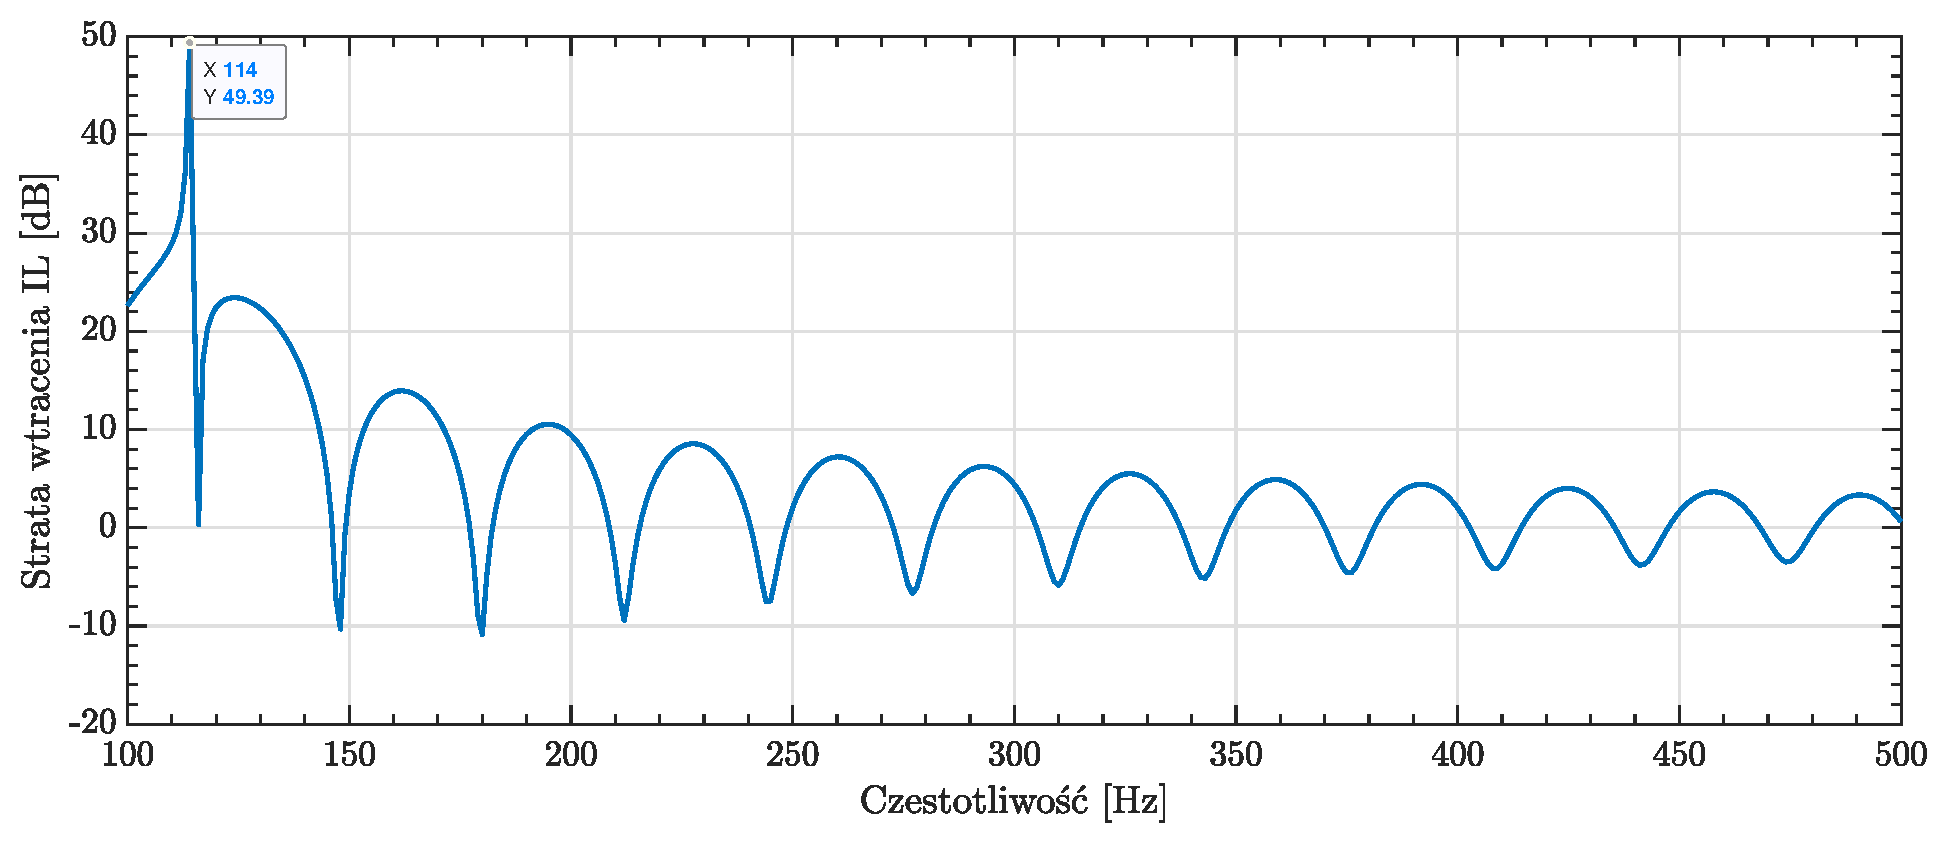
\includegraphics[width=\textwidth]{charIL.eps}
    \caption{Charakterystyka straty wtrącenia $IL(f)$ dla zoptymalizowanego tłumika}
    \label{wykres2}
\end{figure}
\newpage
\subsection{Walidacja dopasowania powierzchni odpowiedzi z interpolowanymi wynikami uzyskanymi metodą omiatania dla $x_1,x_2$}
\par Z metody omiatania wyznaczono 44 punkty wchodzące w dozwolony obszar fizyczny obliczonych z~17 644 par symulacji tłumik--płaski falowód (401 kroków $\Delta f \times$ $8-\Delta x_1\times$ $9-\Delta x_2$). Wyniki następnie interpolowano powierzchnią 2-go stopnia z wyznaczaniem współczynników metodą najmniejszych kwadratów (błąd średniokwadratowy metody: $1,02$ dB). Wynik interpolacji i~współczynniki wielomianu przedstawione są poniżej na \hyperref[wykres3]{wykresie 3}. Maksimum warunkowe znajduje się w punkcie $t_1=1,t_2=1$.
\begin{figure}[htbp!]
    \centering
    \includegraphics[width=0.9\textwidth]{surf_interp.png}
    \caption{Wykres interpolowanej powierzchni odpowiedzi dla metody omiatania}
    \label{wykres3}
\end{figure}
\vspace{-0.8cm}
\section{Wnioski}
\begin{itemize}
\item Maksymalną wartość całkowitej straty wtrącenia na powierzchni odpowiedzi uzyskano dla granicznego przypadku wymiarów tłumika przekraczającego dopuszczalny zakres (\hyperref[plane]{wykres 1.} -- {\color{cyan}punkt niebieski}). Świadczy to o konieczności budowy tłumika z jak najmniejszą szerokością szczeliny pomiędzy wlotem a wylotem kanałów wewnątrz komory. Prawdopodobnie taki dobór wymiarów zaowocowałby również zjawiskiem dyfrakcji, które pozytywnie wpłynęłoby na skuteczność tłumienia.
\item Jest to rozwiązanie gwarantujące najlepsze rezultaty, przy zachowaniu warunku granicznego $x_2>2x_1$. Całkowite usunięcie szczeliny upodobniłoby układ do falowodu i~pozbawiło go jego właściwości. Przy spełnieniu tych założeń, maksymalna strata wtrącenia $IL_{tot}$ wyniosłaby 1,6 dB, dla optymalnego wymiaru całkowitego komory tłumika $x_2=0,344$ m (po znormalizowaniu parametrów: $t_2=-0,64$). Jest to bardzo słaby wynik, lecz należy zaznaczyć, że jest to poziom stosunku mocy akustycznych w~pełnym paśmie.
\item Na \hyperref[wykres2]{wykresie 2.} przestawiono również charakterystykę częstotliwościową straty wtrącenia $IL(f)$ dla zoptymalizowanego tłumika po poprawce nadania szczelinie minimalnej sensownej grubości równej 1 cm. Dla prostoty wykonania realnego tłumika wartości parametrów zaokrąglono w górę do centymetrów: $x_1=0,17$ m, $x_2=0,35$ m.
\item Na charakterystyce widać wyraźne okresowe wzmocnienia i osłabienia tłumienia oraz maksimum obwiedni znajdujące się w peaku tłumienia dla 114 Hz. Jest to typowy charakter dla tłumików akustycznych będących filtrami pasmowymi (dolnoprzepustowymi) i jednocześnie grzebieniowymi, ze względu na okresowy rezonans przy wystąpieniu fali stojącej. Niestety, w wyższym przedziale pasma od około 250 Hz wartość straty wtrącenia $IL$ oscyluje stale wokół 0 dB. Tłumik ten zatem sprawdzi się do tłumienia niskich częstotliwości, szczególnie uciążliwych w podpaśmie $100-140$ Hz.
\end{itemize}
\section{Podsumowanie}
\newcommand{\TikZ}{Ti\textit{k}Z\xspace}
\begin{itemize}
    \item Stworzono autorskie środowisko uruchomieniowe ze składnią do obliczeń straty wtrącenia tłumików akustycznych metodą elementów skończonych wraz z zestawem skryptów pozwalających na wyznaczenie modelu zastępczego tłumika i uzyskanie najbardziej optymalnych parametrów.\\Ma ono szerokie zastosowanie i może wykonać prawie każde z zadań grup (wszystkie osiowo symetryczne), pod warunkiem zmodyfikowania szablonów \texttt{ElmerGrid} ustalając: domeny siatki, współrzędne $X,Y$ domen oraz wektor współrzędnych w funkcji zamiany współrzędnych od parametrów wejściowych: \hyperref[list5]{\texttt{replace.m}}.
    \item Niestety, uzyskany model zastępczy tłumika i jego optymalizacja słabo pokrywa się z~interpolowanymi wynikami uzyskanymi metodą omiatania zmiennymi $x_1, x_2$.\\Każde przybliżanie układu fizycznego modelem zastępczym jest podatne na błędy i~uproszczenia, ponieważ nie przestawia faktycznego rozkładu wartości funkcji celu na powierzchni odpowiedzi pomiędzy węzłami. Zatem, model zastępczy opisany dwuwymiarową powierzchnią 2-go stopnia jest tylko zgrubnym przybliżeniem złożoności obiektu opisanego równaniami różniczkowymi i warunkami brzegowymi.
    \item Grupa wybrała dobranie uboższego, ale jedynego możliwego fizycznie 6-punktowego planu eksperymentu CCI, ale pierwotnym pomysłem grupy było przesunięcie środka obserwacji dla planu CCI i wykonanie dzięki temu nawet planu CCC. Niestety, dobór przedziału parametrów wejściowych zadanych grupie uniemożliwiał taki zabieg. 
    \item Całość projektu wykonano przy użyciu ,,wolnoźródłowych'' narzędzi, ponadto, treść niniejszego sprawozdania, zgodnie z wymaganiami, została sporządzona w systemie składania tekstu \LaTeXe{}, a rysunki w bibliotece graficznej \TikZ.
    \item Obliczenia MES są bardzo ,,zasobożerne'', jednak starano się, by nie występowało w~nich zjawisko aliasingu częstotliwości, stąd mały ich krok dyskretyzacji.\\Dla przykładu, symulacja dla punktów planu CCI zajęła około 6 godzin dla komputera wyposażonego w procesor 4-rdzeniowy Intel Core i5-6300HQ $2,3-3,2$ GHz. Każdy niezauważony błąd przed skończeniem symulacji wymagał uruchomienia ich ponownie.\\Stwierdzono, że nie ma sensu bardzo zagęszczać siatki dla metody omiatania, ponieważ obliczenia zajęłyby na użytym komputerze w przybliżeniu 2 tygodnie. Do takiego zadania wymagany by był klaster obliczeniowy, chociażby Cyfronetu AGH, niestety, grupa nie miała do niego dostępu.
    \item Oszacowano, że na projekt poświęcono około 60 godzin, co w zupełności wyczerpuje i~przekracza wymagania ECTS dotyczące modułu MES w przedmiocie MiNPwA. Starano się, by na każdym poziomie projektu jego realizacja spełniała wymagania opisane w instrukcji, stąd tak długi poświęcony czas, pomimo problematycznego okresu pandemii.
\end{itemize}
\section{Bibliografia}
\renewcommand\labelenumi{[\theenumi]}
\begin{enumerate}
    \item \href{http://home.agh.edu.pl/~iczajka/assets/pliki/MiNPwA2018_2.pdf}{\label{ref1}Konspekt do laboratorium nr 2 z MES MiNPwA}
    \item \href{http://home.agh.edu.pl/~iczajka/assets/pliki/MiNPwA_wyklad1-nup.pdf}{\label{ref2}Wykład z MES dr inż. Ireneusza Czajki}
    \item \href{https://asa.scitation.org/doi/pdf/10.1121/1.1819377}{\label{ref3}R. Ming, J. Pan -- Insertion loss of an acoustic enclosure}
    \item \href{https://www.sciencedirect.com/science/article/pii/S2092678216302618}{\label{ref4}H. Kim, J. Kim, S. Lee, Y. Seo -- A simple formula for insertion loss prediction of large acoustical enclosures using statistical energy analysis method}
    \item \href{http://home.agh.edu.pl/~iczajka/assets/pliki/MiNPwA2018_3.pdf}{\label{ref5}Konspekt do laboratorium nr 3 z MES MiNPwA}
\end{enumerate}
\renewcommand\thesection{\fnsymbol{section}}
\section{Przydział zadań w grupie}
\begin{itemize}
    \item Maja Szydłowska -- stworzenie planu eksperymentu, wyznaczenie przedziału dozwolonego dla parametrów wejściowych, obliczenia transformacji współrzędnych naturalnych na znormalizowane, edycja rozdziału III
    \item Justyna Szymańska -- optymalizacja tłumika, wykonywanie równolegle obliczeń na maszynie wirtualnej Linuxa \texttt{VirtualBox}, napisanie skryptów do stworzenia planu CCI, edycja rozdziału II
    \item Dominika Woźniak -- napisanie kodu do interpolacji wyników planu CCI powierzchnią odpowiedzi, walidacja wyników i ich analiza, zapisanie wniosków w rozdziale IV, stworzenie wykresów i rysunków
    \item Alexander Stefani -- analiza teoretyczna, uruchamianie skryptów na komputerze z systemem Linux, implementacja głównego skryptu oraz metody omiatania, zarządzanie kodem i repozytorium, skład tekstu, autor I i V rozdziału, koordynowanie projektem.
\end{itemize}
\end{document}